\section{Exercise E}
The following tableau are made:
\begin{enumerate}

\item 
$ \forall x (P(x) \to Q(x)), \forall x P(x) \models \forall x Q(x) $ 
\begin{center}
\begin{tikzpicture}

\node {$ \begin{array}{c} \textcolor{red}{1}\; \forall x (P(x) \to Q(x)):\textbf{T} \\ \textcolor{red}{2}\; \forall x P(x):\textbf{T} \\ \textcolor{red}{3}\; \forall x Q(x):\textbf{F} \end{array} $} [sibling distance = 2cm] [level distance=20mm] 
        child {node {$ \textcolor{red}{4}\; Q(c_0):\textbf{F} $} 
            child {node {$ \begin{array}{c} \textcolor{red}{5}\; P(x):\textbf{T} \\ \textcolor{red}{6}\; P(c_0):\textbf{T} \end{array} $}
                child {node {$ \begin{array}{c} \textcolor{red}{7}\; P(x) \to Q(x):\textbf{T} \\ \textcolor{red}{8}\; P(c_0) \to Q(c_0):\textbf{T} \end{array} $} [sibling distance = 6cm]
                    child {node {$ \begin{array}{c} \textcolor{red}{9}\; P(x):\textbf{F} \\ \times \end{array} $}}
                    child {node {$ \begin{array}{c} \textcolor{red}{10}\; Q(x):\textbf{T} \end{array} $} [sibling distance = 4cm]
                            child {node {$ \begin{array}{c} \textcolor{red}{11}\; P(c_0):\textbf{F} \\ \times \end{array} $}}
                            child {node {$ \begin{array}{c} \textcolor{red}{12}\; Q(c_0):\textbf{T} \\ \times \end{array} $}
                        edge from parent node [right, red] {$\to T\;on\; 8$}}
                        edge from parent node [right, red] {$\to T\;on\; 7$}}
                        edge from parent node [right, red] {$\forall T\;on\; 1$}}
                        edge from parent node [right, red] {$\forall T\;on\; 2$}} 
                        edge from parent node [right, red] {$\forall F\;on\; 3$}};

\end{tikzpicture}
\end{center}
It can be seen that the claim holds since all branches in the tableau are closed.
\newpage

\item 
$ \forall x (P(x) \lor Q(x)) \models \forall x P(x), \forall x Q(x) $ 
\begin{center}
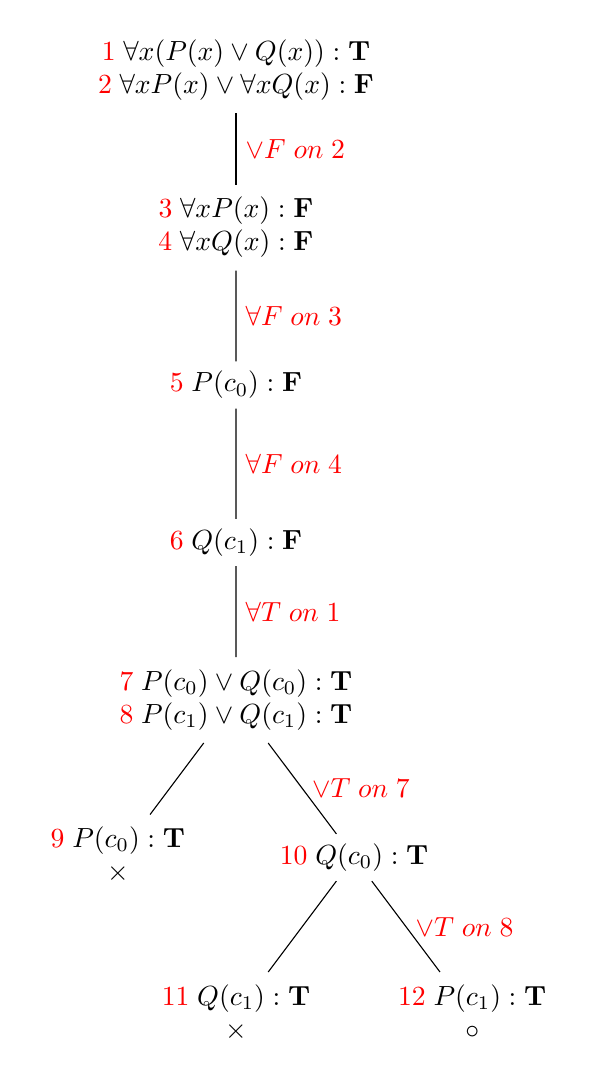
\begin{tikzpicture}

\node {$ \begin{array}{c} \textcolor{red}{1}\; \forall x (P(x) \lor Q(x)):\textbf{T} \\ \textcolor{red}{2}\; \forall x P(x) \lor \forall x Q(x):\textbf{F} \end{array} $} [sibling distance = 2cm] [level distance=20mm] 
        child {node {$ \begin{array}{c} \textcolor{red}{3}\; \forall x P(x):\textbf{F} \\ \textcolor{red}{4}\; \forall x Q(x):\textbf{F} \end{array} $} 
            child {node {$ \textcolor{red}{5}\; P(c_0):\textbf{F} $}
                child {node {$ \textcolor{red}{6}\; Q(c_1):\textbf{F} $}
                    child {node {$ \begin{array}{c} \textcolor{red}{7}\; P(c_0) \lor Q(c_0):\textbf{T} \\ \textcolor{red}{8}\; P(c_1) \lor Q(c_1):\textbf{T} \end{array} $} [sibling distance = 3cm]
                        child {node {$ \begin{array}{c} \textcolor{red}{9}\; P(c_0):\textbf{T} \\ \times \end{array} $}} 
                        child {node {$ \textcolor{red}{10}\; Q(c_0):\textbf{T} $}
                            child {node {$ \begin{array}{c} \textcolor{red}{11}\; Q(c_1):\textbf{T} \\ \times \end{array} $}} 
                            child {node {$ \begin{array}{c} \textcolor{red}{12}\; P(c_1):\textbf{T} \\ \circ \end{array}$}
                                    edge from parent node [right, red] {$\lor T\;on\; 8$}}
                                    edge from parent node [right, red] {$\lor T\;on\; 7$}}
                                    edge from parent node [right, red] {$\forall T\;on\; 1$}}
                                    edge from parent node [right, red] {$\forall F\;on\; 4$}}
                                    edge from parent node [right, red] {$\forall F\;on\; 3$}} 
                                    edge from parent node [right, red] {$\lor F\;on\; 2$}};

\end{tikzpicture}
\end{center}
As it is shown in the tableau method, the claim does not hold because there's an open branch.
\newpage

\item
$ \exists x \forall y P(x,y) \models \forall y \exists x P(x,y) $ 
\begin{center}
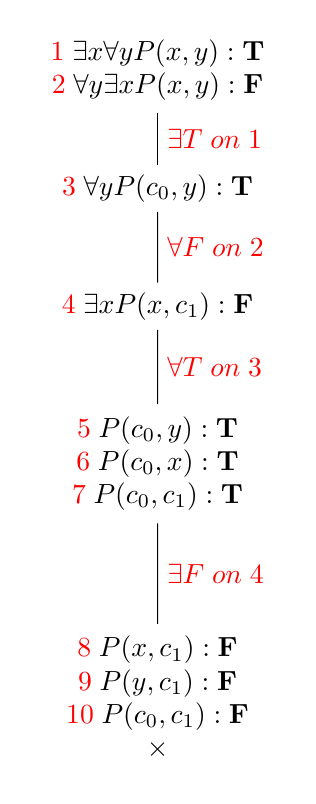
\begin{tikzpicture}

\node {$ \begin{array}{c} \textcolor{red}{1}\; \exists x \forall y P(x,y):\textbf{T} \\ \textcolor{red}{2}\; \forall y \exists x P(x,y):\textbf{F} \end{array} $} [sibling distance = 2cm] 
        child {node {$ \textcolor{red}{3}\; \forall y P(c_0,y):\textbf{T} $} 
            child {node {$ \textcolor{red}{4}\; \exists x P(x,c_1):\textbf{F} $} [level distance=20mm]
                child {node {$ \begin{array}{c} \textcolor{red}{5}\; P(c_0,y):\textbf{T} \\ \textcolor{red}{6}\; P(c_0,x):\textbf{T} \\ \textcolor{red}{7}\; P(c_0,c_1):\textbf{T} \end{array} $} [level distance=30mm] 
                    child {node {$ \begin{array}{c} \textcolor{red}{8}\; P(x,c_1):\textbf{F} \\ \textcolor{red}{9}\; P(y,c_1):\textbf{F} \\ \textcolor{red}{10}\; P(c_0,c_1):\textbf{F} \\ \times \end{array} $}
                                    edge from parent node [right, red] {$\exists F\;on\; 4$}}
                                    edge from parent node [right, red] {$\forall T\;on\; 3$}}
                                    edge from parent node [right, red] {$\forall F\;on\; 2$}} 
                                    edge from parent node [right, red] {$\exists T\;on\; 1$}};

\end{tikzpicture}
\end{center}
As it is shown in the tableau method, the claim holds because of the contradiction between the terms in line 10 and in line 8 which closes the branch.
\end{enumerate}